\documentclass{article}
\usepackage{graphicx}
\graphicspath{{arm/},{pic/},{./}}
\begin{document}
\section*{Beacon Verification}
The mobile unit uses one of the PIC timers to coordinate transmitting of the
UART.  This timer triggers and interrupt, which based on some modulo arithmetic
to create a slower interval, sends a TIMER message to the main loop every eighth
of a second.  The main loop will send a miwi packet containing the current gps string buffer
contents every 8th of a second based on the received message.  In Figure \ref{mobile}
you can see that the timer message is received (it scrolls at 8 events per
second), and correspondly for each one a MiWi packet is transmitted.

The uart interrupt handler simply uses code supplied for the class to send
messages containing up to 4 characters to the main loop.  One alteration made it
so that if there was a newline in the uart receiver, it would send whatever had
been buffered, so that if there ever is a newline, it will be at the end of a
message.  This makes line buffering easier.  The main loop receives the message
and forms full lines.  If they are valid GPS location strings, it will save them
for transmit.  This is visible through the constant activation of the UART
thread throughout the transmitting.

It can be verified in Figure \ref{packets} that the miwi packets contents are a valid
GPS string.  Every 8 packets, you will see that each of the receiver nodes has
transmitted a packet containing what it has perceived as signal strength.

\section*{Node 0 Verification}
Node 0, 1, and 2 are effectively the same code.  The miwi packet handler
triggers if a packet has been received, at which point the function
handle\_miwi will deal with the packet.  If it was a beacon containing a valid
GPS string, the string is saved, the GPS information parsed, and the RSSI value
saved.  Every 8 beacon packets received triggers the node to average the RSSI
values and transmit a packet of its own, containing the average value.  If the
packet was not a GPS string, but contained a node number and a RSSI value, the
value is saved. 

You can see in Figure \ref{node0} that every time an average is computed, a packet is
transmitted.  

This means that each node, listening on its own I2C address, is aware of every
other node's perceived RSSI values, and the ARM board can be connected to any of
them.  In our case, we used node 0.  On the I2C bus, node 0 presents parsed GPS
information

\section*{Arm Verification}
On the ARM, the main logic operates in a giant loop with sequenced events.
First, the I2C thread is used to get GPS and rssi information from Node 0.
Afterwards, the calculation task runs, which is used to estimate coordinates for
the mobile node.   in Figure \ref{node0} that every time an average is computed, a
packet is transmitted.  After that, the filesystem task and LCD task are used to
display data in their respective systems.

In the figures, the GPIO pins are monitored with the logic analyzer, and are
changed to represent the start/stop of a particular task.  0 represents the
filesystem task, 1 represents the LCD task, 2 represents the I2C task,
and 3 represents the calculation task.

In Figure \ref{4tasks}, you can see all four tasks, starting with 2 and 3 (I2C and
calculation), and then the rest of the time is spent updating the filesystem and
LCD display.  Figure \ref{4tasks_2} shows another view of more time, and you can see
the reptition of the four tasks.  Figure \ref{4tasks_close} shows a more zoomed in view
where you can clearly see the I2C task operating before the calculation.

\newpage
\section*{Figures}
\begin{figure}[h]
  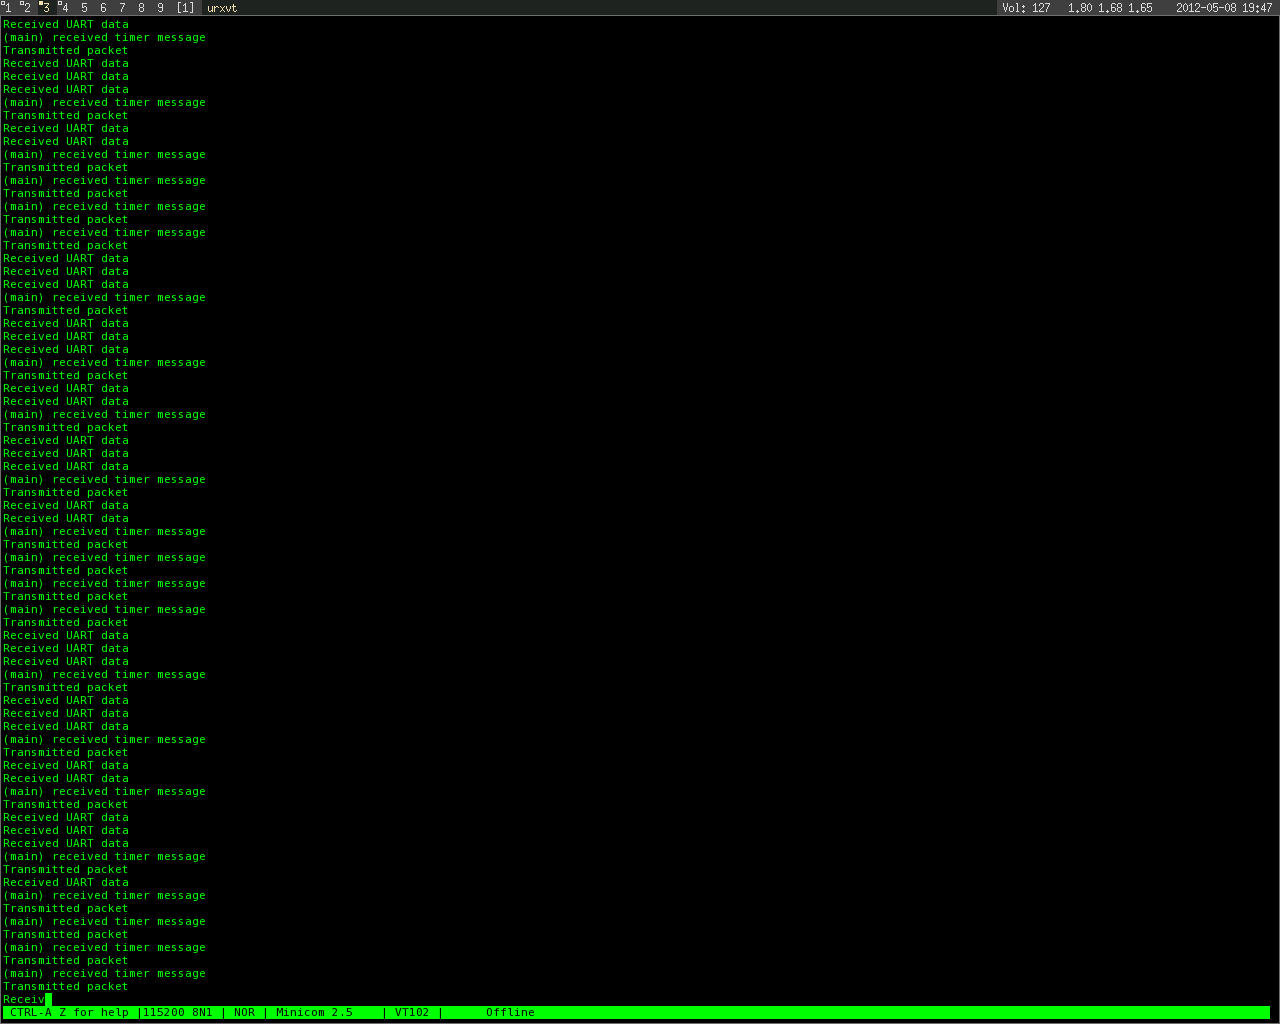
\includegraphics[width=1.1\textwidth]{mobile}
  \caption{UART output of the mobile board}
  \label{mobile}
\end{figure}
\begin{figure}[h]
  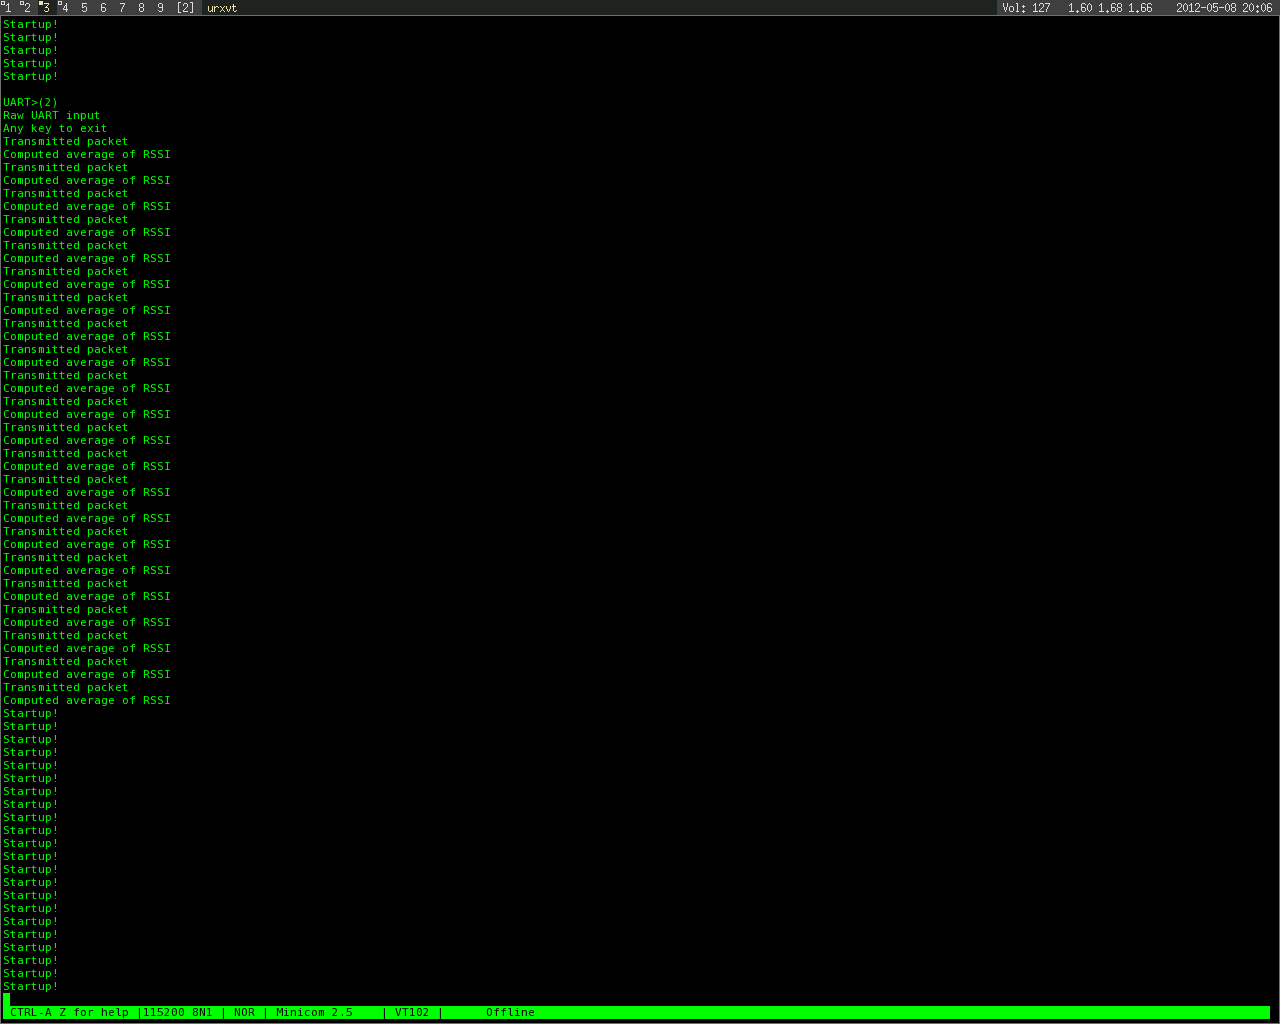
\includegraphics[width=1.1\textwidth]{node0}
  \caption{UART output of Node 0}
  \label{node0}
\end{figure}
\begin{figure}[h] 
  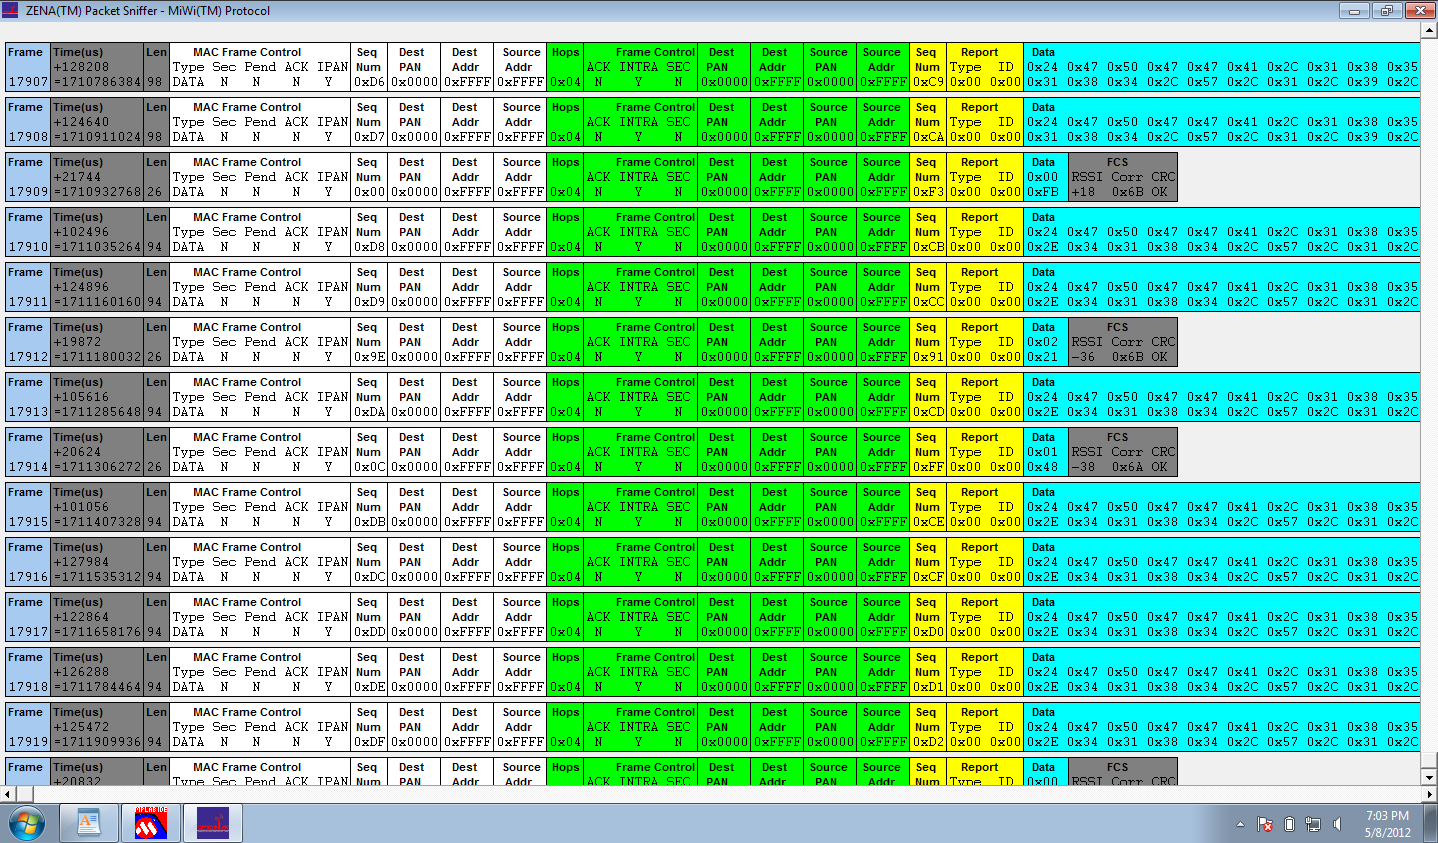
\includegraphics[width=1.1\textwidth]{packets}
  \caption{Packet Capture of all boards}
  \label{packets}
\end{figure}
\begin{figure}[h]
  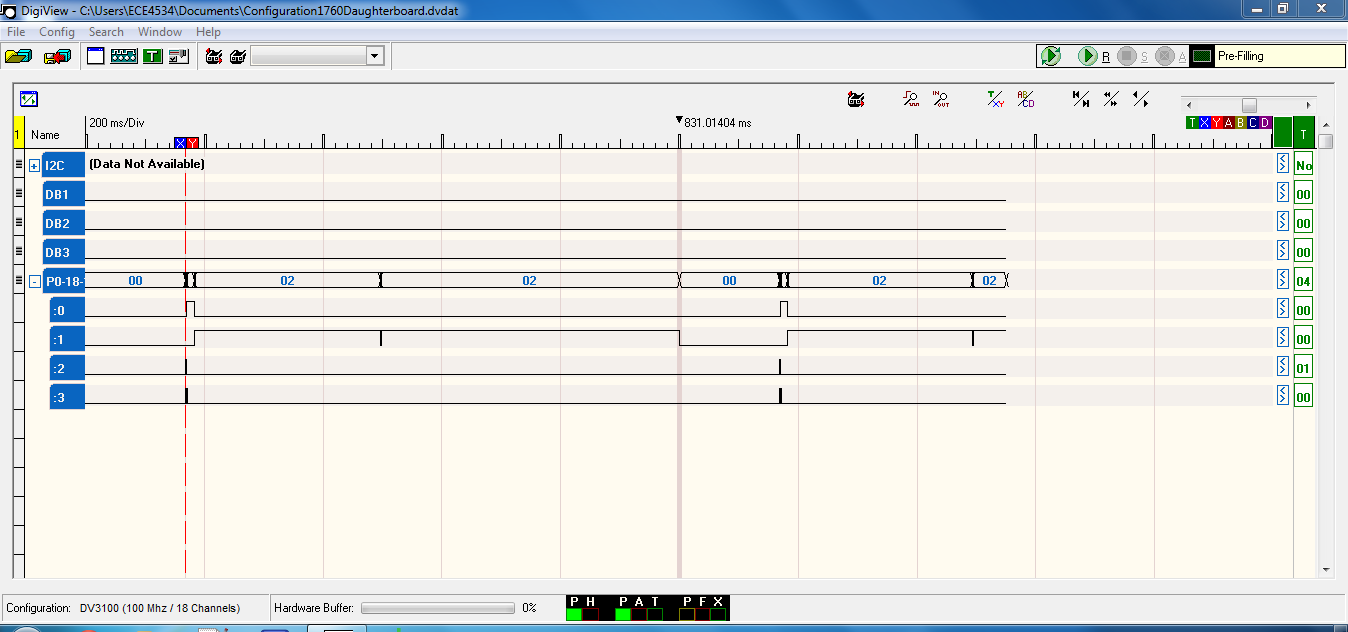
\includegraphics[width=1.1\textwidth]{4tasks}
  \caption{View of the four tasks}
  \label{4tasks}
\end{figure}
\begin{figure}[h]
  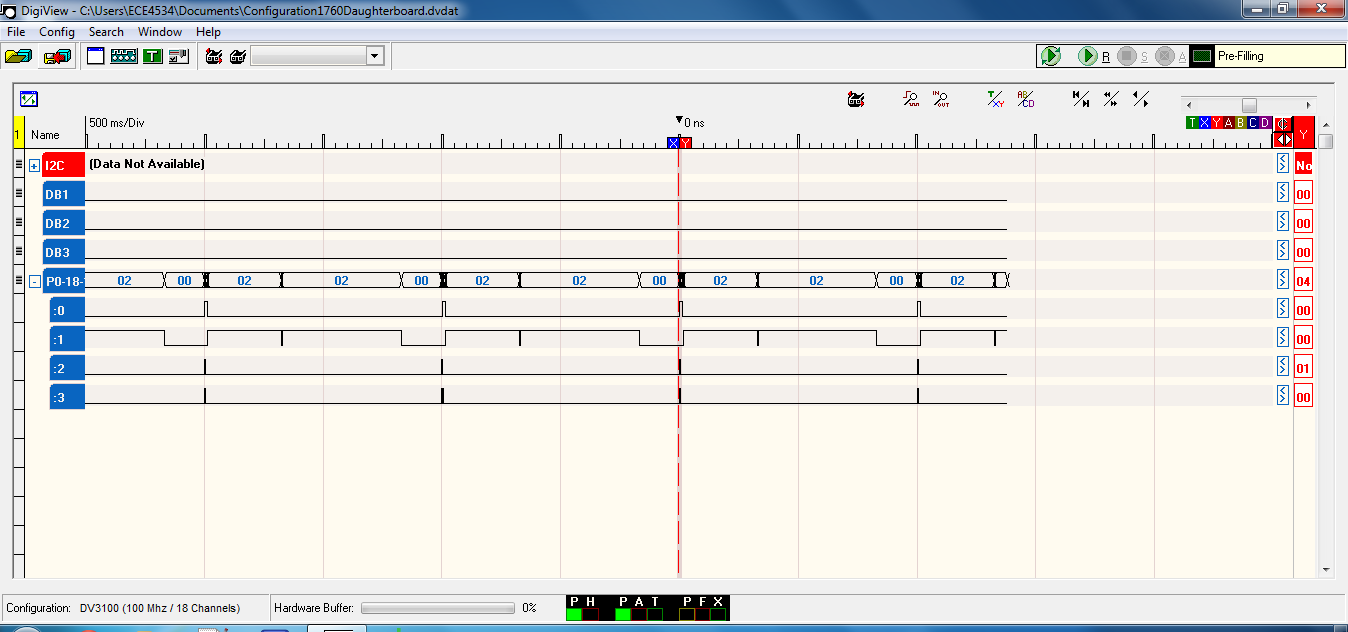
\includegraphics[width=1.1\textwidth]{4tasks_2}
  \caption{View of the four tasks repeating}
  \label{4tasks_2}
\end{figure}
\begin{figure}[h]
  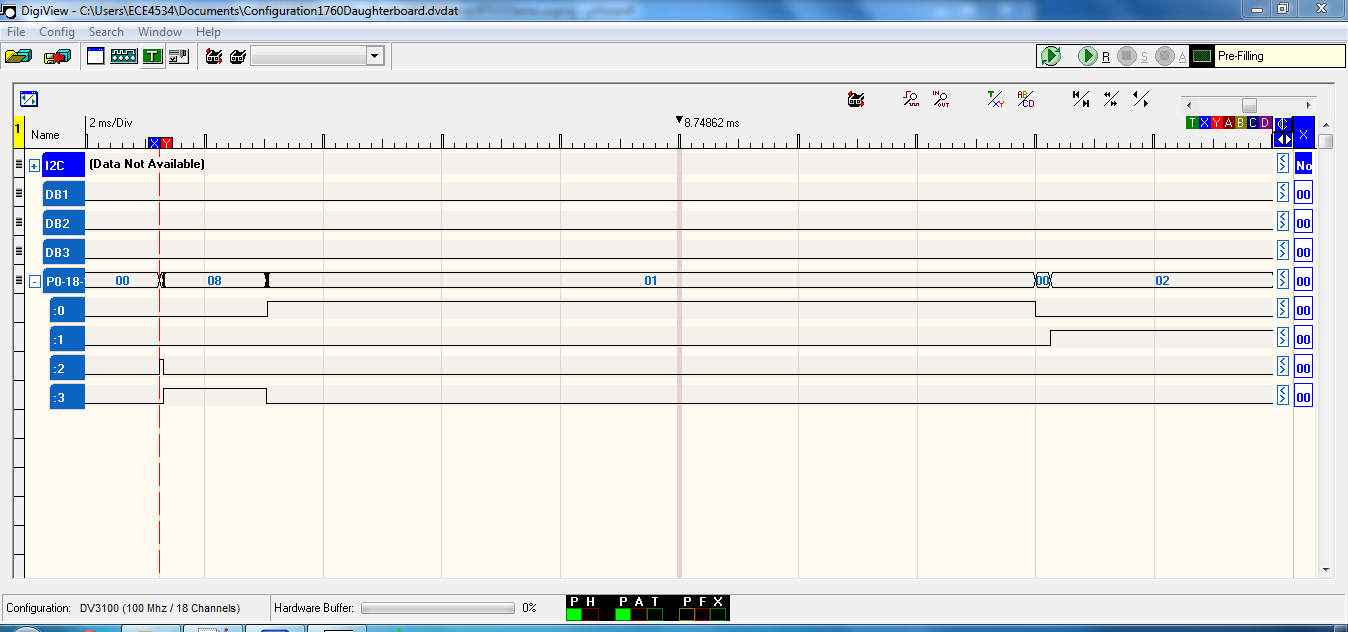
\includegraphics[width=1.1\textwidth]{4tasks_close}
  \caption{Closeup of the first two tasks}
  \label{4tasks_close}
\end{figure}



\end{document}


